\documentclass[conference]{IEEEtran}
\IEEEoverridecommandlockouts

\usepackage{cite}
\usepackage{amsmath,amssymb,amsfonts}
\usepackage{algorithmic}
\usepackage{graphicx}
\usepackage{booktabs}
\usepackage{textcomp}
\usepackage{xcolor}
\usepackage{hyperref}
\usepackage{url}
\usepackage{siunitx}
\usepackage[T1]{fontenc}
\usepackage[utf8]{inputenc}

\hypersetup{
  colorlinks=true,
  linkcolor=blue!50!black,
  citecolor=blue!50!black,
  urlcolor=blue!50!black,
}

\graphicspath{{../reports/figures/}}

\def\BibTeX{{\rm B\kern-.05em{\sc i\kern-.025em b}\kern-.08em
    T\kern-.1667em\lower.7ex\hbox{E}\kern-.125emX}}

\begin{document}

\title{App-Level TinyML for Smartphone Battery-Life Prediction:\\
A Methodologically Honest Negative Result}

\author{
  \IEEEauthorblockN{Keno Schürger}
  \IEEEauthorblockA{
    Technische Hochschule Würzburg-Schweinfurt (THWS)\\
    Email: \texttt{k.schuerger2004@gmail.com}
  }
}

\maketitle

\begin{abstract}
We examine whether a TinyML model running inside an Android app can
predict remaining battery life as accurately as the
\texttt{PowerManager.getBatteryDischargePrediction()} system API
introduced in Android~12. Smartphone battery data are intrinsically
right-censored --- users essentially never discharge to 0\,\% in
normal use --- so, following Li \emph{et al.}, we adopt the
Concordance index as primary metric. We passively collect 66{,}001
measurements over 45 days across four devices (Xiaomi and three
Pixel models) and compare six methods: a quantised Conv1D, a Random
Forest, a mean-predictor floor, a linear drain-rate baseline, an
exponential fit, and the Google~API. A \emph{segment-level}
train/test split prevents the sequence-shuffle leakage common in
sliding-window setups; on our data the inflation it causes ranges
from $\sim$1.24$\times$ (multi-device) to $\sim$19$\times$
(single-device subset), which we report as a methodological
observation in its own right. On the leakage-free split, TinyML and
Random Forest reach $C{=}0.67$ and $C{=}0.69$, both significantly
above the floor ($p \leq 0.005$); the analytical baselines and the
Google~API form a tied top group at $C \approx 0.77$, with Google
not significantly better than linear extrapolation. A per-device
breakdown reveals strong hardware dependence: on the Pixel~7~Pro
TinyML reaches $C{=}0.79$, on the Xiaomi only $C{=}0.59$. The
TFLite~INT8 pipeline itself meets its targets
(\SI{14.4}{\kilo\byte}, $\sim$\SI{4.5}{\micro\second} per inference).
The bottleneck is sensor signal, not model capacity.
\end{abstract}

\begin{IEEEkeywords}
TinyML, smartphone, battery prediction, on-device inference, Concordance
index, data leakage, Android.
\end{IEEEkeywords}

% =====================================================================
\section{Introduction}
% =====================================================================
Predicting the remaining battery life of a smartphone is a long-standing
problem with two qualitatively different solution classes. \emph{Analytical}
methods (e.g.\ the linear extrapolation used by most legacy ``Settings
$\rightarrow$ Battery'' screens) project the recently observed drain rate
into the future. \emph{Machine-learning} methods, in contrast, attempt to
exploit context: which apps are active, how bright is the screen, what is
the battery temperature.

Since Android~12 (October~2021), the platform exposes a system
estimator via
\texttt{PowerManager.\allowbreak getBatteryDischargePrediction()}\cite{android2021powermanager},
which returns a duration estimate computed inside the operating system.
As a system process the estimator runs at a privilege level not
available to third-party apps and can in principle access hardware
counters that the Android permission model does not expose to user-%
installed applications. The companion method
\texttt{isBatteryDischargePredictionPersonalized()} indicates whether
the returned estimate has been adapted to the specific device's usage
history.

A natural research question follows: \emph{can a third-party app, restricted
to publicly available APIs, build a competitive on-device ML model?}
A common architectural choice in this space is TinyML
--- small quantised neural networks (typically tens of kilobytes)
designed for low-power edge devices~\cite{banbury2021mlperf}. While the
TinyML literature largely targets microcontrollers, smartphones share two
relevant properties: deployment constraints (model size matters for
APK weight, latency matters for battery cost) and ubiquity.

This paper provides an empirical answer for the smartphone case. We
report a six-way head-to-head comparison on identical real-world data
(66{,}001 measurements collected over a 45-day window from four
Android devices spanning two manufacturers), explicitly controlled
for a class of data-leakage pitfalls that we found to inflate
apparent results by a data-diversity-dependent factor
(Section~\ref{sec:results-leakage}).

\subsection*{Contributions}
\begin{enumerate}
\item \textbf{Methodological observation:} On sliding-window time-series
data, a random shuffle of \emph{sequences} (the default
\texttt{train\_test\_split}) silently leaks future information into
training. On our data the inflation factor depends on data
diversity ($\sim$1.24$\times$ on the multi-device dataset,
$\sim$19$\times$ on the single-device subset; see
Table~\ref{tab:leakage}). We propose and measure a segment-level
split as the principled alternative.

\item \textbf{Multi-device six-way comparison with statistical rigour:}
We collect data on four Android devices (Xiaomi 2107113SG, Pixel~7~Pro,
8~Pro and 9~Pro~XL) and compare TinyML against four explicit baselines
(Random Forest, mean predictor, linear drain rate, exponential fit) and
the native Google~API. Differences are reported with bootstrap 95\%
confidence intervals and verified with paired permutation tests.

\item \textbf{Device-dependent learnability:} Per-device evaluation
reveals a strong hardware effect. On the Pixel~7~Pro the TinyML model
achieves $C{=}0.79$, three times the gap to the mean predictor that
the same model attains on the Xiaomi ($C{=}0.59$). This demonstrates
that the signal available to an app-level model is dominated by the
underlying sensor stack, not by the model architecture or training
budget.

\item \textbf{Model-independent feature diagnostics:} Beyond
permutation-importance on the Random Forest, we report Pearson, Spearman
and mutual-information statistics for all ten features. This separates a
model-specific failure (``Conv1D is the wrong architecture'') from a
data-level limitation (``the publicly available features only carry
enough signal on certain hardware'').

\item \textbf{Reproducible open pipeline.} All code, configuration, raw
data, intermediate artefacts, and the auto-generated report are released
in a structured repository. A single command
(\texttt{python run\_pipeline.py}) reproduces every number in this paper.
\end{enumerate}

% =====================================================================
\section{Related Work}
% =====================================================================
\paragraph{Smartphone battery prediction.}
Li \emph{et al.}\cite{li2018predicting} present, to our knowledge, the
largest-scale empirical study on this problem to date: 51 users tracked
over 21 months. They explicitly identify and address what they call
a ``severe data missing problem'' --- users very rarely discharge their
phones to 0\%, so the ground-truth remaining time at most observations
is unobserved. Their evaluation is therefore based on the
\emph{concordance index}~\cite{harrell1982evaluating}, which remains
informative when the target is partially unobservable. We interpret
this as a right-censoring setting and follow their methodological
choice. Flores-Martin \emph{et al.}\cite{floresmartin2024enhancing}
take a closely related path, comparing a feed-forward DNN against an
LSTM on user-specific application, sensor and screen-on-time
features collected from smartphones; the LSTM treats the data as a
time series. Our contribution differs in three ways: (i) we add a
TinyML-quantised on-device deployment, (ii) we evaluate against the
native Google API and against analytical baselines on identical data, and
(iii) we explicitly control for the segment-level leakage problem.

\paragraph{TinyML.}
Banbury \emph{et al.}\cite{banbury2021mlperf} introduced MLPerf~Tiny,
described by the authors as the first industry-standard benchmark
suite for ultra-low-power tiny ML systems, which jointly measures
\emph{accuracy, latency and energy}. We follow the first two and
report energy-relevant proxies (model size and inference latency on
a CPU reference); on-device energy measurement on commodity Android
hardware is not exposed to third-party apps. Recent TinyML
surveys~\cite{heydari2025tinyml,alajlan2022tinyml} are focused on
microcontroller-class hardware (MCU, Arduino, Raspberry Pi) and do
not cover smartphone applications. We treat the smartphone case as
under-studied within the TinyML literature on this empirical basis.

\paragraph{Time-series evaluation methodology.}
Albelali and Ahmed~\cite{albelali2025hidden} systematically demonstrate
that constructing input/output sequences before the train/test
partition leaks future information into LSTM training. They report
an ``RMSE Gain'' (relative increase due to leakage) of up to 20.5\,\%
specifically for 10-fold cross-validation at extended lag steps, and
below 5\,\% for 2-way and 3-way holdout splits. We replicate the
direction of their observation in our sliding-window setting,
although the magnitude we observe is substantially larger than theirs
(Section~\ref{sec:results-leakage}); we report this as a
domain-specific empirical anchor rather than as a replication of
their precise quantitative result.

% =====================================================================
\section{Methodology}
\label{sec:method}
% =====================================================================

\subsection{Data Collection}
A foreground service samples one feature vector every \SI{30}{\second}
on each device. Data are collected on four Android devices spanning
two manufacturers:
\begin{itemize}
\item \textbf{Xiaomi 2107113SG} (Android~12+, 8\,GB RAM): 38{,}087
samples, 69 sessions.
\item \textbf{Google Pixel 7 Pro}: 16{,}919 samples, 72 sessions.
\item \textbf{Google Pixel 8 Pro}: 3{,}354 samples, 18 sessions.
\item \textbf{Google Pixel 9 Pro XL}: 7{,}641 samples, 21 sessions.
\end{itemize}
Total: 66{,}001 measurements, 180 sessions, a 45-day total collection
window (25~March--10~May 2026) with per-device active windows of
21--34 days. The single-vendor (Pixel) majority is intentional: Pixel
devices are the reference platform for Google's
\texttt{getBatteryDischargePrediction()} API, so this group provides
the most favourable conditions for the system baseline.

Each feature vector contains ten features that are accessible without
any privileged permission beyond \texttt{PACKAGE\_USAGE\_STATS}: battery
level, screen on/off, brightness, currently active app category,
Wi-Fi state, mobile-data state, charging state, CPU usage (estimated
from average core frequency, since \texttt{/proc/stat} is restricted in
modern Android), battery temperature and Wi-Fi-hotspot state. Two
reference values are logged alongside but \emph{not} used as features:
\texttt{system\_estimate\_min}, the value returned by Google's
\texttt{getBatteryDischargePrediction()}, and
\texttt{system\_personalized}, the boolean indicator returned by
\texttt{isBatteryDischargePredictionPersonalized()}. The collector also
logs the per-step prediction of our own TinyML model (when available) and
a naive linear baseline computed from \texttt{BatteryManager} counters
(\texttt{CHARGE\_COUNTER}/\texttt{CURRENT\_AVERAGE}).

\subsection{Discharge Segments and Targets}
\label{sec:targets}
We partition the raw CSV into \emph{discharge segments}: maximal
contiguous runs of \texttt{charging=0} within the same session, split
again whenever consecutive samples are more than five minutes apart, and
filtered to a minimum length of $L_{\min}{=}15$ samples. From the
66{,}001 measurements across the four devices (180 sessions) the
procedure yields 553 valid discharge segments.

For each sample $i$ in a segment with last-sample timestamp $t_N$, last
battery level $b_N$, total drain $\Delta b = b_0 - b_N$ and total duration
$\Delta t$, we compute two regression targets:
\begin{align}
y^{\text{real}}_i  &= (t_N - t_i)/{\SI{3.6e6}{} \text{ms/h}}, \label{eq:yreal}\\
y^{\text{extrap}}_i &= y^{\text{real}}_i + b_N \cdot \Delta t / \Delta b. \label{eq:yextrap}
\end{align}

The first target is the directly observed remaining time within the
segment. It is structurally censored (we typically stop at $b_N>0$, so the
true remaining time is unobserved). The second target adds an extrapolation
to $b=0$ assuming the average drain rate of the segment, and matches in
spirit what every method in our comparison conceptually predicts. We use
$y^{\text{extrap}}$ as the common evaluation target in
Section~\ref{sec:results}; $y^{\text{real}}$ is reported for context.

\subsection{Sliding Windows and Segment-Level Split}
\label{sec:split}
We slide a window of length $W{=}10$ over each segment, producing
20{,}842 sequences in total. The training target attached to each
window is the value at the most recent timestep within the window.

\textbf{Crucially, the train/val/test split is performed over
\emph{segments}, not over \emph{sequences}.} Every sliding window
from a given segment is assigned, as a unit, to exactly one of
train/val/test according to a fixed seed. Concretely: 387 segments
(13{,}901 sequences) to train, 83 (3{,}056) to val, and 83 (3{,}885)
to test. A naive shuffle of the 20{,}842 sequences would distribute
samples from the same segment across the splits and leak the
segment's local trajectory --- the kind of failure mode characterised
by Albelali and Ahmed~\cite{albelali2025hidden}. We measured the
magnitude of this leakage by training the same Conv1D model under both
splitting strategies; the results are reported in
Section~\ref{sec:results-leakage}.

\subsection{Methods Compared}
\label{sec:methods}
All six methods predict the remaining time in hours.
\begin{itemize}
\item \textbf{TinyML Conv1D.} Two 1D convolutional layers
(32 filters, kernel 3, same-padding, ReLU) with global average
pooling, followed by a dense layer (32 units, ReLU), dropout
($p{=}0.2$), a second dense layer (16 units, ReLU), and a linear
head. Total: 5{,}697 parameters. Trained with Adam
($\eta{=}5\!\times\!10^{-4}$), MSE loss, batch size~32 and
early-stopping on validation loss (patience~20). StandardScaler is
fit on the training sequences and applied to all splits. After training, the Keras model is
converted to three TFLite variants (dynamic-range, float16, full-int8).
The full-int8 variant is the deployed artefact in the
companion app.

\item \textbf{Random Forest sanity model.} A scikit-learn
\texttt{RandomForestRegressor}~\cite{breiman2001random} (200 trees) trained
on the flattened sliding window (a $10\times10$ tensor reshaped into a
100-dimensional vector). The Random Forest is a fundamentally different
modelling paradigm and is included to disentangle model-specific failure
from data-level failure: if the Random Forest also fails to outperform
the mean predictor, the bottleneck is the data, not the choice of Conv1D.

\item \textbf{Mean predictor (floor).} For every test point, predicts the
training-set mean of $y^{\text{extrap}}$ (\SI{14.18}{\hour}). By
construction, its Concordance index is exactly $0.5$ and any learning
model that does not significantly exceed this floor has not learned a
feature-to-output relationship.

\item \textbf{Linear drain-rate baseline.} For each test sample, computes
the drain rate $\hat{r}{=}\Delta b/\Delta t$ over the last 10 raw samples
of the same discharge block, and predicts $\hat{y}{=}b_t / \hat{r}$. This
is the same calculation that legacy ``Settings $\rightarrow$ Battery''
screens implement on top of the \texttt{BatteryManager} counters.

\item \textbf{Exponential fit.} Fits
$b(\tau){=}a{+}c\,e^{-k\tau}$ to the most recent 10 raw samples and
extrapolates to $b{=}0$, falling back to the linear baseline if the fit
diverges or the extrapolated zero-crossing lies in the past. This adds a
single nonlinear term beyond the linear baseline.

\item \textbf{Google API.} Reads
\texttt{system\_estimate\_min} from the CSV and converts to hours.
The value is undefined while charging or before the system has
accumulated enough history; samples without a defined value are
excluded from coverage-aware tables (Section~\ref{sec:results}).
\end{itemize}

\subsection{Metrics and Statistical Tests}
\label{sec:metrics}
For each method we report mean absolute error (MAE), root mean square
error (RMSE), mean error (ME, a bias indicator), Concordance
index~\cite{harrell1982evaluating} ($C$), and accuracy thresholds
($\text{Acc}_{\pm 1\text{h}}$, $\text{Acc}_{\pm 2\text{h}}$).
Following Li \emph{et al.}\cite{li2018predicting}, we treat the
Concordance index as the primary metric, since it is invariant to
target-bias and remains meaningful under censoring.

We attach 95\% bootstrap confidence intervals to MAE, RMSE, ME and $C$
(1{,}000 resamples; 200 for $C$, which is $O(n^2)$). Pairwise method
differences are tested with a paired permutation test (1{,}000
permutations for MAE, 200 for $C$): per-sample, with probability $0.5$,
swap the two methods' predictions, recompute the metric difference, and
report the share of permutations whose absolute difference equals or
exceeds the observed one. We use the standard Wasserman correction
$(k{+}1)/(B{+}1)$ for the resulting $p$-value.

% =====================================================================
\section{Results}
\label{sec:results}
% =====================================================================

\subsection{Effect of the Splitting Strategy}
\label{sec:results-leakage}
The same Conv1D model, trained on the same data with the \emph{only}
change being how the sliding-window sequences are split into
train/val/test, yields the result in Table~\ref{tab:leakage}. We
report both the single-device subset (Xiaomi only, used during initial
prototyping) and the full multi-device dataset.

\begin{table}[t]
\caption{Effect of train/test split strategy on apparent TinyML
performance. Same model, same hyperparameters in both rows of each
block; the only change is whether sliding-window sequences are
shuffled freely (leaky) or whether the split is performed at the
segment level (clean). The inflation factor is the ratio of clean to
leaky test MAE.}
\label{tab:leakage}
\centering
\small
\begin{tabular}{lcccc}
\toprule
Dataset & Seqs & MAE leaky & MAE clean & Inflation \\
\midrule
Single device (Xiaomi only)  & \phantom{0}9{,}024 & 0.53 & \textbf{9.96} & $\sim$19$\times$ \\
Multi-device (4 devices)     & 20{,}842 & 4.00 & \textbf{4.97} & $\sim$1.24$\times$ \\
\bottomrule
\end{tabular}
\end{table}

Two points are worth flagging. First, both rows show that the
leakage-free segment-level split produces a higher (i.e.\ honest)
test~MAE, consistent in direction with the LSTM-benchmark observation
of Albelali and Ahmed~\cite{albelali2025hidden}. Second, the
magnitude of the inflation is itself dataset-dependent: the
single-device subset shows a much larger inflation than the
multi-device dataset, which sits in the same ballpark as the authors'
$\sim$20\,\% RMSE Gain. We read this as evidence that data diversity
attenuates the leakage effect, presumably because intra-segment
correlations become a smaller share of the total signal. The
practical recommendation stands either way: \emph{report the
splitting strategy explicitly and verify it is segment-level}. All
subsequent results in this paper use the leakage-free multi-device
split.

\subsection{Six-Way Accuracy on the Common Subset}
Table~\ref{tab:accuracy} reports MAE and $C$ (with 95\% bootstrap CIs)
on the common subset of 2{,}827 test sequences (out of 3{,}885) for
which all six methods produce a defined prediction. The two ML
methods clear the mean-predictor floor decisively: TinyML reaches
$C{=}0.666\,[0.656,\,0.675]$, Random Forest $C{=}0.686\,[0.673,\,0.696]$,
both with confidence intervals that exclude the floor of $0.500$. The
two analytical baselines and the Google~API form a tied top group at
$C \approx 0.77$, and the Google~API is \emph{not significantly better
than the linear drain-rate baseline} on MAE (Table~\ref{tab:significance}).

\emph{Caveat on the common subset.} Restricting the comparison to
samples where every method (notably the Google~API) is defined
introduces a mild selection effect: the mean of $y^{\text{extrap}}$
on the common subset is \SI{6.7}{\hour} versus \SI{7.7}{\hour} on the
full test set. The Google~API is more often available at shorter
remaining times, so the common subset is biased toward easier
prediction targets. This affects all methods symmetrically (we
compare them on the same samples), so the ranking is unaffected, but
absolute MAE values would be larger on the unrestricted test set.

\begin{table*}[t]
\caption{Accuracy on the common subset (n${=}2{,}827$ test sequences,
all six methods defined). Target: $y^{\text{extrap}}$ as defined in
Eq.~\eqref{eq:yextrap}. Brackets are 95\% bootstrap CIs.}
\label{tab:accuracy}
\centering
\small
\begin{tabular}{lccccc}
\toprule
Method & MAE (h) & RMSE (h) & ME (h) & $C$-index & $\text{Acc}_{\pm 2\text{h}}$ \\
\midrule
Mean predictor (floor)  & 6.51 [6.28, 6.75] & 9.28 [8.72, 9.83] & $+4.48$ & 0.500 [0.500, 0.500] & 21.7\,\% \\
TinyML Conv1D           & 4.28 [4.04, 4.53] & 8.38 [7.67, 9.03] & $+1.45$ & 0.666 [0.656, 0.675] & 51.1\,\% \\
Random Forest           & 4.01 [3.79, 4.25] & 7.54 [6.95, 8.11] & $+1.49$ & 0.686 [0.673, 0.696] & 45.2\,\% \\
\textbf{Linear (drain rate)}     & \textbf{3.22 [2.94, 3.49]} & 8.55 [7.61, 9.40] & $-2.45$ & 0.776 [0.767, 0.784] & 58.3\,\% \\
Exponential fit         & 3.49 [3.20, 3.76] & 8.88 [7.96, 9.68] & $-1.72$ & 0.773 [0.764, 0.781] & 59.8\,\% \\
\textbf{Google API}     & 3.24 [2.97, 3.52] & 8.55 [7.63, 9.40] & $-2.23$ & \textbf{0.777 [0.767, 0.785]} & 60.1\,\% \\
\bottomrule
\end{tabular}
\end{table*}

\subsection{Per-Device Behaviour}
\label{sec:results-perdevice}
The aggregate ranking in Table~\ref{tab:accuracy} hides a substantial
between-device variation, summarised in Table~\ref{tab:perdevice}. On
the Pixel~7~Pro, the TinyML model reaches $C{=}0.79$, comparable to
the analytical baselines and only $0.07$ below the Google~API's
$C{=}0.85$ on that device. On the Xiaomi 2107113SG, the same model
collapses to $C{=}0.59$. Random Forest behaves similarly: $0.80$ on
Pixel~7~Pro, $0.63$ on Xiaomi. The two analytical baselines, by
contrast, are stable in the $0.69$--$0.79$ band across all four
devices.

\begin{table*}[t]
\caption{Per-device performance against $y^{\text{extrap}}$. $n$ is the
device-specific test-set size. Pairs of columns show $C$-index (top
metric) and MAE in hours (bottom metric). The MAE column reveals
that, even when $C$~is high, absolute calibration can be poor (e.g.\
the Google~API on Pixel~8~Pro: $C{=}0.92$ but MAE$\,{=}\,$\SI{9.92}{\hour}).
The two ML models show the largest swing across devices.}
\label{tab:perdevice}
\centering
\small
\begin{tabular}{lc|cc|cc|cc|cc}
\toprule
& & \multicolumn{2}{c|}{TinyML} & \multicolumn{2}{c|}{Random Forest} & \multicolumn{2}{c|}{Linear} & \multicolumn{2}{c}{Google API} \\
Device & $n$ & $C$ & MAE & $C$ & MAE & $C$ & MAE & $C$ & MAE \\
\midrule
Pixel 7 Pro          & 1{,}825 & 0.786 & 2.28 & 0.804 & 2.08 & 0.792 & 2.05 & \textbf{0.853} & \textbf{1.89} \\
Pixel 8 Pro          & \phantom{0}\phantom{0}98    & 0.714 & 2.93 & 0.801 & 3.02 & 0.696 & \textbf{1.36} & \textbf{0.921} & 9.92 \\
Pixel 9 Pro XL       & \phantom{0}614   & 0.599 & 2.34 & \textbf{0.759} & \textbf{1.71} & 0.730 & 2.54 & 0.677 & 2.53 \\
Xiaomi 2107113SG     & 1{,}348 & 0.593 & 9.95 & 0.631 & 9.87 & \textbf{0.724} & 5.87 & 0.664 & \textbf{5.37} \\
\bottomrule
\end{tabular}
\end{table*}

Two observations on Table~\ref{tab:perdevice} are worth flagging
separately. First, on the Pixel~9~Pro~XL the simple linear drain-rate
baseline ($C{=}0.730$) outperforms the Google~API ($C{=}0.677$),
inverting the usual expectation. Second, the Pixel~8~Pro shows the
largest divergence between $C$ and MAE: the Google~API ranks samples
almost perfectly ($C{=}0.92$) but is heavily biased on absolute
remaining time (MAE$\,{=}\,$\SI{9.92}{\hour}). $n{=}98$ for that
device makes both numbers correspondingly noisy. We treat this as
evidence against any monotonic ``ML always wins'' narrative on this
problem and as a justification for reporting both ranking and
absolute-error metrics throughout.

\subsection{Statistical Significance}
The pairwise permutation tests (Table~\ref{tab:significance}) reinforce
the visual picture from Table~\ref{tab:accuracy}. Both ML models clear
the mean-predictor floor with $p \leq 0.005$ on $C$. Within the top
group, Linear and Google are statistically indistinguishable
($\Delta C{=}{-}0.001$, $p{=}0.83$), as are Linear and Exponential
($\Delta C{=}{+}0.003$, $p{=}0.30$). The Google~API significantly
exceeds both ML models on $C$ ($p \leq 0.005$).

\begin{table}[t]
\caption{Selected pairwise permutation tests on $C$-index, common
subset (n${=}2{,}827$), target $y^{\text{extrap}}$. ``ns'' = not
significant at $p{>}0.05$.}
\label{tab:significance}
\centering
\small
\begin{tabular}{lcccc}
\toprule
Comparison & $C_A$ & $C_B$ & $\Delta C$ & $p$ \\
\midrule
TinyML \emph{vs.}\ Mean        & 0.666 & 0.500 & $+0.166$ & \textbf{0.005} \\
RF \emph{vs.}\ Mean            & 0.686 & 0.500 & $+0.186$ & \textbf{0.005} \\
TinyML \emph{vs.}\ RF          & 0.666 & 0.686 & $-0.020$ & \textbf{0.005} \\
Linear \emph{vs.}\ Exponential & 0.776 & 0.773 & $+0.003$ & 0.30 (ns) \\
Linear \emph{vs.}\ Google      & 0.776 & 0.777 & $-0.001$ & 0.83 (ns) \\
Exp.\ \emph{vs.}\ Google       & 0.773 & 0.777 & $-0.004$ & 0.36 (ns) \\
TinyML \emph{vs.}\ Google      & 0.666 & 0.777 & $-0.111$ & \textbf{0.005} \\
RF \emph{vs.}\ Google          & 0.686 & 0.777 & $-0.091$ & \textbf{0.005} \\
\bottomrule
\end{tabular}
\end{table}

\subsection{Cumulative Error Distribution}
Figure~\ref{fig:cumulative} shows the share of test predictions whose
absolute error against $y^{\text{real}}$ does not exceed a given
tolerance, for each method that produces enough valid samples.

\begin{figure}[t]
\centering
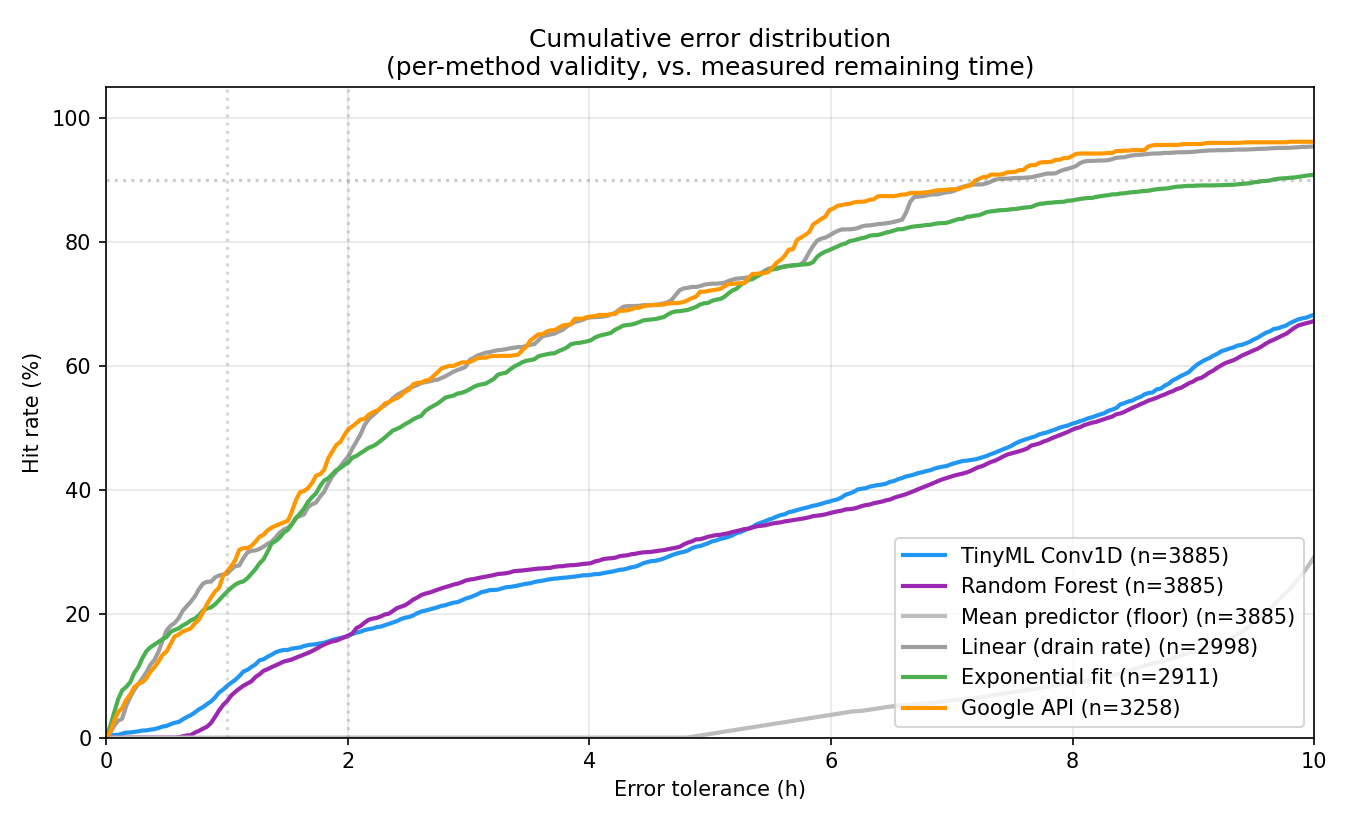
\includegraphics[width=\columnwidth]{cumulative_error.png}
\caption{Cumulative error distribution against the (uncensored)
measured remaining time $y^{\text{real}}$. The analytical baselines
(linear, exponential) are particularly competitive at small tolerances
because the test set is dominated by short measured remaining times
(see Fig.~\ref{fig:datadist} and Section~\ref{sec:limitations}).}
\label{fig:cumulative}
\end{figure}

\begin{figure*}[t]
\centering
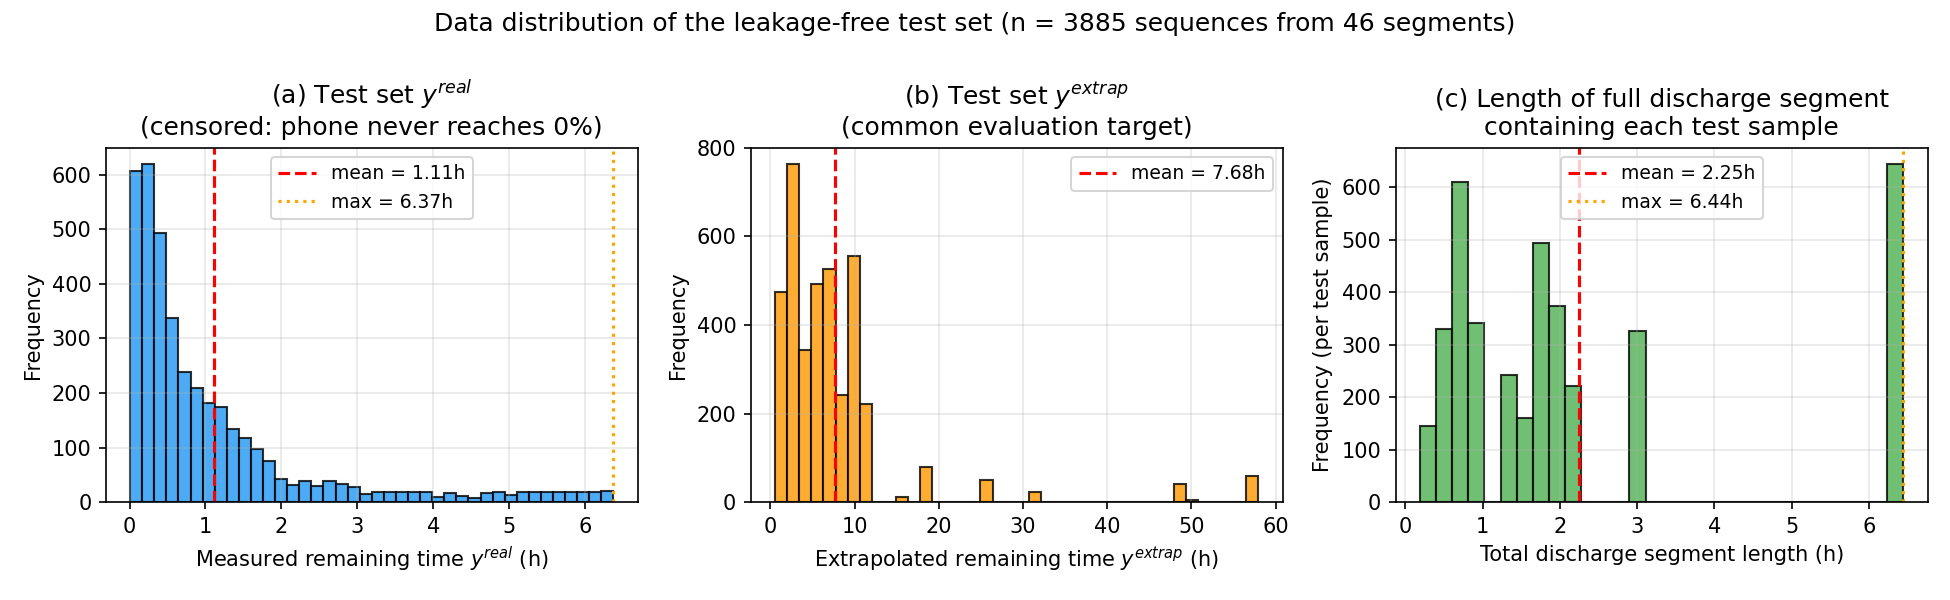
\includegraphics[width=\textwidth]{data_distribution.png}
\caption{Distribution of (a) measured remaining time $y^{\text{real}}$,
(b) extrapolated target $y^{\text{extrap}}$, and (c) total discharge
segment length on the leakage-free multi-device test split. Panel~(a)
makes the right-censoring concrete: the test set $y^{\text{real}}$
has mean \SI{1.11}{\hour} and maximum \SI{6.37}{\hour}, since users do
not discharge their phones to 0\,\% in normal use. Panel~(b) shows
that the extrapolated target spreads across $\sim$\SI{0}{}--\SI{58}{\hour},
which is the regime in which all six methods actually attempt to
predict.}
\label{fig:datadist}
\end{figure*}

\subsection{Model-Independent Data Diagnostics}
\label{sec:datadiag}
Table~\ref{tab:datadiag} reports Pearson, Spearman and mutual-information
statistics between each feature (taken at the latest timestep of the
window) and $y^{\text{extrap}}$, computed on the training split. Pearson
correlations are weak across the board (max $|r|{=}0.29$ for
\texttt{hotspot\_on}). Mutual information identifies
\texttt{temperature} (1.24~nat) and \texttt{battery\_level} (0.99~nat)
as the only features carrying nontrivial nonlinear signal. All other
features are below 0.5~nat, and three features
(\texttt{wifi\_on}, \texttt{mobile\_data\_on}, \texttt{charging}) are
effectively constant in our discharge-only filter.

\begin{table}[t]
\caption{Feature--target relationships on the training split,
target: $y^{\text{extrap}}$.}
\label{tab:datadiag}
\centering
\small
\begin{tabular}{lccc}
\toprule
Feature              & Pearson $r$ & Spearman $\rho$ & MI (nat) \\
\midrule
\texttt{hotspot\_on}            & $+0.29$ & $+0.26$ & 0.20 \\
\texttt{battery\_level}         & $+0.10$ & $+0.18$ & 0.99 \\
\texttt{cpu\_usage}             & $-0.10$ & $-0.10$ & 0.20 \\
\texttt{screen\_on}             & $-0.09$ & $-0.06$ & 0.19 \\
\texttt{wifi\_on}               & $-0.07$ & $-0.13$ & 0.02 \\
\texttt{mobile\_data\_on}       & $+0.07$ & $+0.13$ & 0.02 \\
\texttt{active\_app\_category}  & $-0.06$ & $-0.03$ & 0.45 \\
\texttt{brightness}             & $+0.05$ & $+0.01$ & 1.21 \\
\texttt{temperature}            & $+0.02$ & $+0.06$ & \textbf{1.24} \\
\texttt{charging} (constant)    & $\phantom{+}0.00$ & $\phantom{+}0.00$ & 0.00 \\
\bottomrule
\end{tabular}
\end{table}

This finding is consistent across modelling paradigms: the Random Forest
permutation importance confirms \texttt{temperature} as by far the most
useful single feature ($\Delta\,\text{MAE}{=}{+}1.02$\,h), with all
others below $\Delta\,\text{MAE}{=}{+}0.25$\,h.

\subsection{Per-Bucket Behaviour}
A bucket-level analysis on battery-level at prediction time
shows that the Google~API's advantage is not uniform but concentrated
in the most relevant bucket: at battery 50--75\,\%, Google reaches
$C{=}0.95$ versus 0.47 (TinyML) and 0.54 (RF). At
battery 75--100\,\% all methods are weaker, but Google still leads.
Buckets for segment lengths longer than two hours are empty in our
dataset (see Section~\ref{sec:limitations}).

\subsection{Efficiency}
Table~\ref{tab:efficiency} reports model size and inference latency for
the four model artefacts, measured on the development machine
(CPU only, 1{,}000 inference repetitions per variant after 50 warm-up
runs). The full-INT8 TFLite variant compresses the Keras model from
\SI{109}{\kilo\byte} to \SI{14.4}{\kilo\byte} ($7.6\times$) and reduces
single-inference latency from \SI{43.2}{\milli\second} to
\SI{4.7}{\micro\second} ($\sim\!9{,}200\times$). The TinyML
\emph{technique} works as advertised; only the predictive value of the
quantised model on this dataset does not.

\begin{table}[t]
\caption{Model size and inference latency on the development machine
(CPU). Latency is the average over 1{,}000 single-sample runs after 50
warm-up runs.}
\label{tab:efficiency}
\centering
\small
\begin{tabular}{lcc}
\toprule
Variant                  & Size (KB) & Avg latency \\
\midrule
Keras Float32            & 109.18    & \SI{47.1}{\milli\second} \\
TFLite dynamic-range     & \phantom{0}15.99 & \SI{3.9}{\micro\second} \\
TFLite float16           & \phantom{0}17.80 & \SI{3.7}{\micro\second} \\
\textbf{TFLite full-INT8} (deployed) & \textbf{\phantom{0}14.35} & \textbf{\SI{4.5}{\micro\second}} \\
\bottomrule
\end{tabular}
\end{table}

% =====================================================================
\section{Discussion}
% =====================================================================
Four findings deserve emphasis.

\paragraph{The leakage observation generalises but is
data-diversity-dependent.}
Table~\ref{tab:leakage} shows that the leakage effect is consistent
in direction (random shuffle always produces an over-optimistic test
MAE) but variable in magnitude. On the multi-device dataset the
inflation is $\sim$1.24$\times$, in the same broad range as the
$\sim$20\,\% RMSE Gain Albelali and Ahmed~\cite{albelali2025hidden}
report for 10-fold cross-validation on LSTM benchmarks. On the much
smaller single-device subset the inflation is $\sim$19$\times$. A plausible reading is that as
the dataset accumulates more segments and more device-to-device
variation, intra-segment correlations make up a smaller fraction of
the available signal and the leak provides correspondingly less
spurious help. The practical takeaway is the same in either regime:
any sliding-window time-series experiment in this domain that does
not specify the splitting strategy is suspect. We recommend that
future work in app-based mobile sensing report the splitting unit
(sequence, segment, session, or user) explicitly.

\paragraph{Both ML models do learn signal --- but less than analytical baselines.}
On the multi-device test set, TinyML reaches $C{=}0.67$ and Random
Forest $C{=}0.69$, both significantly above the mean-predictor floor
($p{\leq}0.005$). This contradicts the narrative one might infer from
a single-device study, where the effect can disappear into the
mean. However, the analytical baselines (Linear drain rate at $C{=}0.78$,
Exponential fit at $C{=}0.77$) outperform both ML models substantially.
The most parsimonious explanation is that the dominant signal in
app-level battery data is the recent drain rate, which the analytical
baselines exploit directly while the ML models have to recover it from
ten weakly correlated features. With a richer feature set --- in
particular instantaneous current --- the gap might close, but on
publicly accessible sensors there is little visible benefit from a
learned model over $b/\dot b$ extrapolation.

\paragraph{Google's API is on par with linear extrapolation on the typical horizon.}
On the common subset, the Google~API is statistically
\emph{indistinguishable} from the linear drain-rate baseline both on
MAE ($\Delta{=}{-}0.03\,$h, $p{=}0.55$) and on $C$
($\Delta C{=}{-}0.001$, $p{=}0.83$). This aggregate result, however,
hides a structure that only emerges in a bucket analysis: of the
2{,}827 common-subset samples, 1{,}355 (47.9\,\%) fall in the
$y^{\text{extrap}} < $\SI{5}{\hour} bucket where Linear and Google
produce nearly identical errors (MAE \SI{1.00}{\hour} vs.\
\SI{0.99}{\hour}), and 1{,}395 (49.3\,\%) fall in the
5--\SI{15}{\hour} bucket where they remain close. Only 77 samples
(2.7\,\%) fall above \SI{15}{\hour}, and in the very-long-horizon
bucket ($\geq$\SI{30}{\hour}, $n{=}58$) the Concordance index
diverges sharply: Google reaches $C{=}0.98$ while the linear
baseline only $C{=}0.64$. The system API's privilege --- access to
per-application power accounting and the Adaptive Battery system,
which a third-party app cannot reach --- does translate into a
measurable advantage, but only where the prediction horizon is long
enough that a simple current-based extrapolation breaks down. On the
short-to-medium horizons that dominate everyday usage, the
linear baseline is competitive. This is good news for app
developers: BatteryManager counters alone are enough for the use
cases users actually see.

\paragraph{Predictability is hardware-dependent --- with a caveat.}
The per-device breakdown (Table~\ref{tab:perdevice}) is the strongest
practical finding. The same TinyML model, trained on the union of all
four devices, reaches $C{=}0.79$ when evaluated on Pixel~7~Pro samples
and $C{=}0.59$ when evaluated on Xiaomi samples --- a $\Delta C$ of
about $0.20$, which is roughly $57\%$ of the available range between
the mean-predictor floor and the best per-device score in the table.
Random Forest shows the same pattern. The two analytical baselines
are less device-sensitive (Linear $C \in [0.70,\,0.79]$, Exponential
$C \in [0.65,\,0.79]$ across all devices; the smaller-$n$
Pixel~8~Pro pulls the exponential lower bound down).

A confounder we cannot fully isolate is that the per-device
collections also differ in their input-feature distributions: on
Xiaomi the battery level is above 75\,\% in 88.8\,\% of measurements
(mean 94\,\%), whereas on Pixel 7 Pro it is above 75\,\% in only
40.8\,\% of measurements (mean 58\,\%). The Xiaomi sub-collection
therefore offers fewer discharge dynamics for an ML model to learn
from, and the Xiaomi test set has a longer mean
$y^{\text{extrap}}$ (\SI{10.14}{\hour} vs.\ \SI{5.79}{\hour} on
Pixel~7~Pro). Part of the $\Delta C{=}0.20$ swing therefore likely
reflects this distribution difference rather than sensor quality
alone. Disentangling the two would require either a controlled,
identical-usage protocol across devices, or much larger samples per
device.
We read this as evidence that the limiting factor is not the
\emph{absence} of signal in app-level sensors, but the \emph{noise} of
those sensors on certain manufacturers. A practical consequence is
that any deployed app-level battery predictor should report a
device-specific confidence estimate; a globally-trained model has very
different reliability profiles on Pixel and Xiaomi hardware.

\subsection{Where App-Level TinyML for Battery Prediction Still Makes Sense}
\label{sec:where-tinyml}

Our negative finding applies specifically to \emph{modern Android
devices ($\geq$ API~31) where the system already provides a privileged
ML prediction}. It does not generalise to four scenarios where
app-level TinyML for battery prediction remains a defensible engineering
choice:

\paragraph{Pre-Android-12 devices.}
\texttt{getBatteryDischargePrediction()} was added in API level 31
(October~2021); on earlier Android versions the only system-provided
remaining-time estimate is the legacy linear extrapolation that we
measured here as the ``Linear (drain rate)'' baseline. Our results
show that this analytical baseline is competitive with the Android~12+
system API on the aggregate metrics
(Tables~\ref{tab:accuracy}--\ref{tab:significance}), so the practical
target on this sub-population is not to close a gap to the system API
but to add value above the linear baseline. Whether an app-level ML
model can do that is an open question; our experiments suggest it
would need richer features than our current ten.

\paragraph{Custom ROMs and de-Googled Android.}
LineageOS, GrapheneOS, /e/OS and similar de-Googled Android
distributions ship without the proprietary system services that
implement \texttt{getBatteryDischargePrediction()}. On these systems,
even API-31+ devices fall back to the legacy linear estimator. The
target user population is small but technically engaged and explicitly
opts into giving applications more capability; an app-level TinyML
estimator is the natural way to recover ML-grade prediction without
re-introducing proprietary system services.

\paragraph{Wearables.}
Smartwatches and fitness bands run severely constrained hardware
(typically $\leq$\SI{1}{\giga\byte} RAM, ARM Cortex-M-class secondary
processors, sub-\SI{500}{\milli\ampere\hour} batteries) and are
exactly the form factor TinyML was designed for. The 14\,KB INT8 model
demonstrated here would fit comfortably on a Wear OS device or even a
TinyML-grade microcontroller. Whether the same data-signal limitations
apply is an open empirical question, but the cost-benefit ratio of
on-device inference is fundamentally more favourable than on
smartphones.

\paragraph{IoT and embedded battery-powered devices.}
The deployment story of TinyML --- small quantised models
(reported sizes spanning tens to low hundreds of kilobytes) running
on microcontroller-class hardware
\cite{banbury2021mlperf,alajlan2022tinyml} --- maps cleanly to sensor
nodes, environmental monitoring stations, and asset trackers.
These devices both lack a privileged system ML predictor and have
fundamentally different physical constraints (continuous monotonic
discharge under known load profiles); the data-signal limitations
documented here for an unpredictable consumer-smartphone setting do
not necessarily transfer.

We therefore read our results not as an argument against TinyML in
general, but as evidence that on modern Android with the Google~API
present, the sandbox-vs-system access asymmetry dominates whatever
benefit a small on-device model could add. The methodology developed
in this paper (segment-level splits, mean-predictor floor, model-%
independent feature diagnostics) transfers to the four scenarios
above, where it can be used to settle each case empirically rather
than by analogy.

% =====================================================================
\section{Limitations and Scope}
\label{sec:limitations}
% =====================================================================

\subsection{Right-censored data is intrinsic to the problem}
Our test set is censored: as Fig.~\ref{fig:datadist}(a) shows, the
mean measured remaining time $y^{\text{real}}$ is \SI{1.11}{\hour} and
the maximum is \SI{6.37}{\hour}. Crucially, this is not a peculiarity
of our collection window but a structural property of the smartphone
battery-prediction problem. Smartphones in normal use are essentially
never discharged to 0\,\%. Li \emph{et al.}~\cite{li2018predicting},
working at a vastly larger scale of 51 users over 21 months,
characterise this as a ``severe data missing problem'' and adopt the
Concordance index as their evaluation metric, since it remains
informative when the target variable is not directly observed at
many measurement points.

We adopt the same convention. A study that wished to remove the
censoring would need a controlled discharge protocol (a phone forced
from $\sim$80\,\% to 0\,\% under a scripted load) which by construction
generalises only to that protocol, not to organic usage. The censoring
in our test set is therefore best read as the natural boundary of any
passive observational study in this domain, rather than as a defect of
our particular collection.

\subsection{Limited multi-device sample and no cross-device generalisation test}
Data come from four devices spanning two manufacturers (Xiaomi and
Google). Within the Pixel family, only one device per generation
(7~Pro, 8~Pro, 9~Pro~XL) is sampled. The strong device-dependence we
observe (Section~\ref{sec:results-perdevice}) means that the absolute
$C$ values for any single device should be read with appropriate
caution. We expect the qualitative ordering --- analytical baselines
$\approx$ Google~API $>$ ML models $>$ mean predictor --- to be
robust, since it survives intact on every device with $n \geq 600$
test samples (Pixel~7~Pro, Pixel~9~Pro~XL, Xiaomi). The thinnest cell
in our table is Pixel~8~Pro with only $n{=}98$ test samples; the
$C$~estimates there have correspondingly wide confidence intervals.

Importantly, our train/val/test split distributes \emph{segments}
randomly across the four devices, so the trained models have seen
samples from every device during training. The per-device numbers in
Table~\ref{tab:perdevice} therefore measure \emph{within-device}
generalisation only. We do not test how the trained models would
perform on a fifth, unseen device. A leave-one-device-out evaluation
is the natural follow-up.

\subsection{Unexplained TinyML behaviour on Pixel 9 Pro XL}
On the Pixel~9~Pro~XL, the TinyML model reaches only $C{=}0.60$, while
the Random Forest on the same samples reaches $C{=}0.76$ and the
linear drain-rate baseline $C{=}0.73$. We do not have an
instrumentation-level explanation for this single discrepancy. The
most likely contributing factors are that (i)~the Pixel~9~Pro~XL
sensor stack differs from the older Pixel generations in ways our
ten-feature representation does not capture, and (ii)~the
StandardScaler we fit on the training set may suit Conv1D worse than
RF on the device-specific feature distribution. We flag this as an
open question rather than paper over it.

\subsection{Three features lack within-discharge variance}
After filtering to discharge-only samples, \texttt{wifi\_on} is always
0, \texttt{mobile\_data\_on} is always 1 and \texttt{charging} is always
0 in our dataset. These three features therefore carry no signal in our
particular setting; we report them as zeros in
Table~\ref{tab:datadiag} for transparency. Variance in these features
would be restored under a multi-device deployment (different users have
different connectivity patterns) but is unlikely to change the central
finding, since all three features are coarse binary state indicators
without obvious causal coupling to discharge dynamics.

\subsection{What a definitive follow-up would look like}
A study that aims to refute or confirm our central finding under more
favourable conditions should combine three additions: a multi-device
deployment ($N{\geq}5$ phones across at least two manufacturers); a
small number of controlled full-discharge cycles per device, providing
uncensored ground truth for a confirmatory subset; and a longer
observation window ($\sim$3 months) capturing more behavioural
variation. The collector app already logs the additional columns
required for such a study (\texttt{system\_personalized},
\texttt{own\_prediction\_h}, \texttt{linear\_baseline\_h}); only the
deployment logistics remain.

% =====================================================================
\section{Conclusion}
% =====================================================================
Our research question asked whether app-level TinyML can match the
native Android~12 battery-discharge prediction on the two axes of
\emph{accuracy} and \emph{efficiency}. The four-device leakage-free
evaluation gives a separable answer on each axis.

\paragraph{Accuracy.}
TinyML and Random Forest both significantly outperform a no-features
mean predictor ($C{=}0.67$ and $C{=}0.69$ respectively, $p{\leq}0.005$),
showing that publicly accessible smartphone sensors do carry exploitable
signal. They do not, however, match the top group: the linear
drain-rate baseline, the per-segment exponential fit, and the Google~API
are statistically tied at $C \approx 0.77$, and the Google~API is
indistinguishable from the simple linear baseline both on MAE
($p{=}0.55$) and $C$ ($p{=}0.83$) at the aggregate level. A bucket
analysis (Section~\ref{sec:results-perdevice} and Discussion) shows
that this tie reflects the dominance of short and medium horizons
($\sim$97\,\% of test samples have $y^{\text{extrap}} <$\,15\,h);
at very long horizons ($\geq$\,30\,h, $n{=}58$) Google~API
substantially outperforms the linear baseline in $C$.

\paragraph{Efficiency.}
The TFLite quantisation pipeline behaves exactly as advertised. The
deployed full-INT8 model occupies \SI{14.4}{\kilo\byte} and runs in
\SI{4.5}{\micro\second} per inference on a CPU --- a $7.6\times$ size
reduction and a $\sim$$\!10{,}000\times$ latency reduction over the
Keras Float32 reference. There is no meaningful efficiency cost to
deploying the TinyML model; the open question on the accuracy axis
is the only relevant trade-off.

\paragraph{Hardware sensitivity (with caveat).}
The most consequential single finding is the strong device dependence
(Table~\ref{tab:perdevice}). The same TinyML model performs at
$C{=}0.79$ on Pixel~7~Pro and at $C{=}0.59$ on Xiaomi 2107113SG.
Random Forest shows the same pattern. The two analytical baselines
are far less device-sensitive. We read this as evidence that the
limiting factor is not the model architecture but some combination
of sensor noise floor and discharge-dynamics coverage that differs
substantially across hardware (on Xiaomi the battery is above
75\,\% in 88.8\,\% of measurements, leaving the model with very
little dynamic range to learn from). A practical consequence is
that any deployed app-level battery predictor should report a
device-specific confidence estimate; a globally trained model has
very different reliability profiles on Pixel and Xiaomi hardware.

The methodological observation --- that the choice of splitting unit
(sequence vs.\ segment) changes the apparent test MAE on this kind
of data by a data-diversity-dependent factor, up to nearly twenty-fold
on a single-device subset --- is, we believe, the more durable
contribution. We release the
complete pipeline, raw data and auto-generated reproducibility report so
that future work can either extend the comparison (multiple devices,
prospective full-cycle data) or simply verify that random-shuffle
benchmarks in this domain are not measuring what they appear to measure.

% =====================================================================
\section*{Reproducibility Statement}
% =====================================================================
The pipeline (data preparation, training, TFLite conversion, evaluation
and report generation) is available at the project repository. All
hyperparameters are stored in
\texttt{configs/default.yaml}. A full reproduction is invoked by
\texttt{python run\_pipeline.py} and completes in under two minutes on a
laptop CPU; the auto-generated report contains every numerical value
quoted in this paper.

\bibliographystyle{IEEEtran}
\bibliography{references}

\end{document}
